
In this section, we present our point-based-pruning and index-based-pruning
skyline computation algorithms. Point-based-pruning strategy is
our first attempt to formulate a pruning-based algorithm and guarantees
correct result with or without a broadcast index.
%useful
%when MBRs of the index do intersect as in typical R-Tree structure.
Index-based-pruning generally provides better performance by performing
early pruning. We present two index-pruning strategies here.
%but requires that the MBRs of index do \emph{not} intersect.
The algorithms utilize the R-Tree index and allocation
method described in previous section to build a pruning region to
eliminate unwanted data records. Point-based-pruning skyline algorithm
is explained and followed by index-based-pruning algorithm.
%In addition, to simplify our demonstration, we
%first consider 2-dimensional skyline. Later we show how our
%approach can be easily extended to higher dimensions.

%Since a pruning region is the core of solution, we defined it
%here.

\begin{definition}[Pruning Region]
%A region in the space
%$R = D_1 \times D_2 \times ... \times D_n$ that is dominated by
%a subset of $P$ that has been examined so far.
Given the data space defined by $D_1 \times D_2 \times ... \times D_n$,
where $D_i$ is the data domain of attribute $i$,
a pruning region is a pair of a pivot point and an ordered list of
preference specifiers $(p, \sigma)$ that specifies a region of the data
space that has been dominated by a subset of the data-set. As
defined in Section~\ref{sec-prelim}, $\sigma_i$ is one of the values in
$\{min, max\}$.
\end{definition}

A pivot point, denoted by $p$ here, is a n-dimensional point in the
n-dimensional data space that defines the bounds of a pruning region.
The bounds is defined by the list of preference specifiers. For each
attribute $i$, if $\sigma_i = min$, then $p_i$ is the lower bound
of the pruning region for $i$th dimension and the region extends to
the maximal value for $i$th dimension. Similarly, if $\sigma_i = min$,
then $p_i$ is the lower bound and extends to minimal value of data
dimension. Pivot point and pruning region is illustrated in
Figure~\ref{fig:rtree_pr_2d} and \ref{fig:rtree_pr_3d}. Pruning regions
are illustrated as the gray regions and bounded by pivot points $b$ and
$d$. As illustrated, a pruning region is a region of n-dimensional
space (or a n-dimensional box) that has been dominated by $p$ and can be
ignored in the upcoming broadcast data stream.

\begin{corollary}\label{co:pivot_point}
The pivot point of a rectangle dominates all points of the rectangle.
\end{corollary}

\begin{proof}
Given a pivot point, $p$, of a rectangle, $r$, for all attribute $i$,
if $\sigma_i = min$ then $p_i = r.min_i$, if $\sigma_i = max$ then
$p_i = r.max_i$. This implies that the pivot point has the best value
for all attributes in the rectangle, therefore no points can dominate it
and it dominates all points of the rectangle except for itself.
\end{proof}

\begin{figure}[!h]
\label{fig:rtree_pr}
\centering
\subfigure[2-D with preference specifiers (min, min)]{
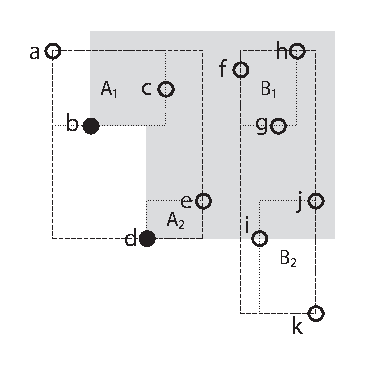
\includegraphics[width=1.6in]{Figures/rtree_pr2.eps}
\label{fig:rtree_pr_2d}
}
\subfigure[3-D with preference specifiers (min, min, max)]{
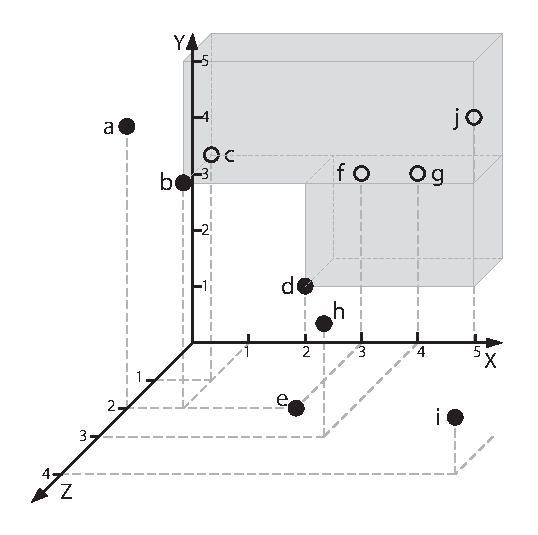
\includegraphics[width=1.6in]{Figures/rtree_pr_3d.eps}
\label{fig:rtree_pr_3d}
}
\caption{Pruning region with pivot points b and d}
\end{figure}


\subsection{Point-Based Skyline Pruning}

To compute the skyline, a pruning region is progressively
augmented as more data records are examined. The algorithm keeps
track of a list of candidate skyline points, $S$, and a pruning
region that is the union of pruning region of $S$. As the pruning
region grows, any $p$ in $S$ that is inside the pruning region is
removed and any new MBR received from the broadcast cycle that is
inside the pruning region is ignored. At the end of the algorithm,
points in $S$ that are not removed are returned as skyline.

Skyline computation is illustrated in
Algorithm~\ref{alg:PBSkyline}. At the beginning of the algorithm,
the client does not have any candidate skyline points; therefore,
the pruning region, $R$, is null ($R =$ {\o}).
In this state, the client cannot prune any R-Tree MBR and
therefore must stay tuned into the channel for the first index bucket
broadcasted on the channel. The client follows a series of index
buckets to the first data segment.
When a data segment is reached, the client does:
\begin{enumerate}
\item Download all data points from the data segment.
\item Compute skyline points, $S_0$, using any existing skyline algorithm
        (NL, BNL, NN, BBS).
\item For each point in $S_0$, compute a pruning region, $R'$, and and remove
    all points in $S$ covered by $R'$.
\item For each $R'$, $R = R \cup R'$
\item Add each point in $S_0$ to $S$.
\end{enumerate}
This repeats until the entire space is inside the pruning region.

Note that the points found in each data segment are only candidate skyline
points since there could data broadcasted later
that dominate the earlier candidate points. If a candidate point
$p_2$ dominates earlier point $p_1$, then $p_1$ is removed from
$S$ and the pruning region is enlarged by the later point $p_2$.
%Algorithm~\ref{alg:PBSkyline} ends when there is no more MBR in
%the broadcast cycle that is outside the pruning region.

ComputePruneRegion() in Algorithm~\ref{alg:PBSkyline} is described
next.
%Note that Algorithm~\ref{alg:PBSkyline} utilizes
%ComputePruneRegion(), which is listed in
%Algorithm~\ref{alg:ComputePruneRegion1}. ComputePruneRegion in
%Algorithm~\ref{alg:ComputePruneRegion1} computes a pruning region
%from a list of candidate skylines points, $S$, based on the
%preference specifiers, $\sigma$. The algorithm loops through each
%point, $s$ in the list, $S$, computes the pruning region for $s$
%and union to the final pruning region. The algorithm returns the
%total pruning region after all points are processed.

\begin{algorithm}
\algsetup{linenosize=\small,linenodelimiter=. }
\caption{Point-Based Skyline($\sigma$)} \label{alg:PBSkyline}
\begin{algorithmic}[1]

\STATE $S \gets$ \o
\STATE $R \gets$ \o
\STATE $index \gets$ search first index bucket
\STATE $queue.enqueue(index.pairs(mbr, time))$
\WHILE{$queue$ is not empty}
    \STATE $bucket \gets GetBucket(queue.dequeue)$
    \IF{$bucket$ is index bucket}
        \FORALL{$pair(mbr, time)$ in $bucket$}
            \IF{$pair$ is not in $pruneRegion$}
                \STATE $queue.enqueue(pair)$
            \ENDIF
        \ENDFOR
    \ELSE
        \STATE $S_0 \gets ComputeSkyline(bucket, \sigma)$
        \STATE $R' \gets ComputePruneRegion(S_0, \sigma)$
        \STATE $Prune(S, R')$
        \STATE $Prune(queue, R')$
        \STATE $R \gets R \cup R'$
        \STATE $S \gets S \cup S_0$
    \ENDIF
\ENDWHILE \RETURN $S$
\end{algorithmic}
\end{algorithm}

%\begin{algorithm}
%\algsetup{linenosize=\small,linenodelimiter=. }
%\caption{ComputePruneRegion($S$, $\sigma$)}
%\label{alg:ComputePruneRegion1}
%\begin{algorithmic}[1]
%
%\STATE $totalR \gets$ \o \FORALL{$p$ in $S$}
%    \STATE $tempR \gets$ ($-\infty$ to $\infty$) for all dimensions
%    \FOR{$i = 0$ to $n$}
%        \IF{$\sigma[i] = MIN$}
%            \STATE $tempR \gets tempR \bigcap (\infty \bigcup ... \bigcup (s[i]~to~\infty)_i \bigcup ... \bigcup \infty $)
%        \ELSE
%            \STATE $tempR \gets tempR \bigcap (\infty \bigcup ... \bigcup (min(D_i)~to~s[i])_i \bigcup ... \bigcup \infty $)
%        \ENDIF
%    \ENDFOR
%    \STATE $totalR \gets totalR \bigcup tempR$
%\ENDFOR \RETURN $totalR$
%\end{algorithmic}
%\end{algorithm}

\subsubsection{Pruning and Pruning Region}
Here we describe pruning region computation and pruning strategy listed in
Algorithm~\ref{alg:PBSkyline}.

%The formulation of a pruning region depends on a pivot point, here we denote
%it with $p$, and the preference specifiers
%of the attributes of the data. For each axis (attribute) of the data space,
%the preference could be either MIN or MAX. For an axis $i$ with MIN specifier,
%the pruning space is from $p.i$ to $\infty$ (or maximum value for the attribute).
%Similarly, for the axis with MAX specifier, the pruning space is from $p.i$ to
%$-\infty$ or minimum value of the attribute. For data of positive value, the
%minimum value would be 0.

To determine if a point $q$ is covered (should be pruned) by a pruning
region, all attributes of the point has to be checked against the pivot
$p$ of the pruning region. The condition for a point to be covered is that
all attributes of point $q$ is inside the pruning region. For a point to
be covered, each attribute $i$ satisfy one of the following:
\begin{enumerate}
  \item If $\sigma_i$ = MIN, then $q_i \geq p_i$.
  \item If $\sigma_i$ = MAX, then $q_i \leq p_i$.
\end{enumerate}

To determine if an index bucket is covered by a pruning region and should be
ignored when computing skyline as in Point-Based Skyline discussed previously,
we need to determine if the MBR of the index bucket is covered. To do so, we
need to determine the pivot point of the MBR according to the preference
specifiers. Based on Corollary~\ref{co:pivot_point}, if the pivot
point of a pruning region dominates the pivot point of the MBR, then the
index bucket can be pruned and ignored, since the pivot point of the MBR
dominates the entire bucket.
Following the definition of a rectangle defined in
Section~\ref{sec:wireless_broadcast},
a MBR is covered by a pruning region if its pivot is covered by the pruning
region as illustrated by Figure~\ref{fig:pruning}. A pruning region is
illustrated in gray and
defined by pivot point $p$ with the skyline query specifiers of
$(X = min, Y = max)$. MBR $A$ can be pruned since its pivot $p_1$ falls
inside the pruning region, while although MBR $B$ is partially covered by
the pruning region, it can not be pruned since its pivot, $p_2$, does
not fall inside the pruning region, in other words $p$ dominates $p_1$, but
does not dominate $p_2$.

\begin{figure}[h]
\begin{center}
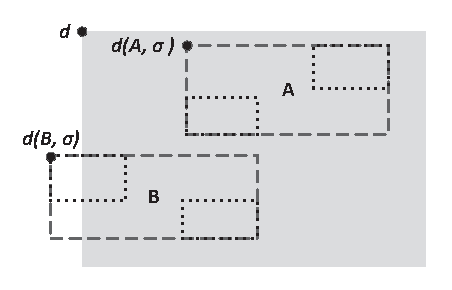
\includegraphics[width=2.5in]{Figures/pruning.eps}
\caption{\small Pruning region defined by $p$ and preference specifier
$(X = min, Y = max)$ and MBRs A and B.}
\label{fig:pruning}
\end{center}
\end{figure}

%\subsubsection{MIN and MAX Attributes}
%In two dimensional skyline when we consider both MIN and MAX
%skyline specifier, there are totally four possibilities. Let x,
%and y be the two attributes of interest, the four possible skyline
%queries we can make out of the two attributes are (MIN $x$, MIN
%$y$), (MIN $x$, MAX $y$), (MAX $x$, MIN $y$), and (MAX $x$, MAX
%$y$). Similar to the (Min $x$, and Min $y$) case, the algorithm
%progressively builds pruning region from the minimal bounding box
%of the index tree and data points received from the broadcast
%program.

%The pruning region orientation differs slightly for each case.
%Given a candidate skyline point $p$, the pruning region for an MIN
%attribute, $x$, would span from $p.x$ to positive infinity. In
%other words the range of the pruning region for the attribute
%%attribute would have pruning region span from 0, to $p.x$, [0,
%$p.x$], for data that does not include negative values or from
%negative infinity to $p.x$, ($-\infty$, $p.x$], for data that
%contains negative values.

%\begin{figure}[ht]
%\centering

%\subfigure[Subfigure 1 caption]{
%   \includegraphics[width=0.5in] {skyline_minx_miny.pdf}
%   \label{fig:subfig1}
% }

% \subfigure[Subfigure 2 caption]{
%   \includegraphics[width=0.5in] {skyline_minx_maxy.pdf}
%   \label{fig:subfig2}
% }

% \subfigure[Subfigure 3 caption]{
 %  \includegraphics[scale=0.5] {skyline_maxx_maxy.pdf}
   %\label{fig:subfig3}
% }


%\label{myfigure}
%\caption{Global figure caption}
%\end{figure}

\begin{comment}
\begin{figure}[h]
\begin{center}
\includegraphics[width=2.5in]{Figures/skyline_minx_miny.pdf}
\caption{\small MIN $x$, MIN $y$ and pruning region.
\label{fig:skyline_minx_miny}}
\end{center}
\end{figure}

\begin{figure}[h]
\begin{center}
\includegraphics[width=2.5in]{Figures/skyline_minx_maxy.pdf}
\caption{\small MIN $x$, MAX $y$ and pruning region.
\label{fig:skyline_maxx_maxy}}
\end{center}
\end{figure}

\begin{figure}[h]
\begin{center}
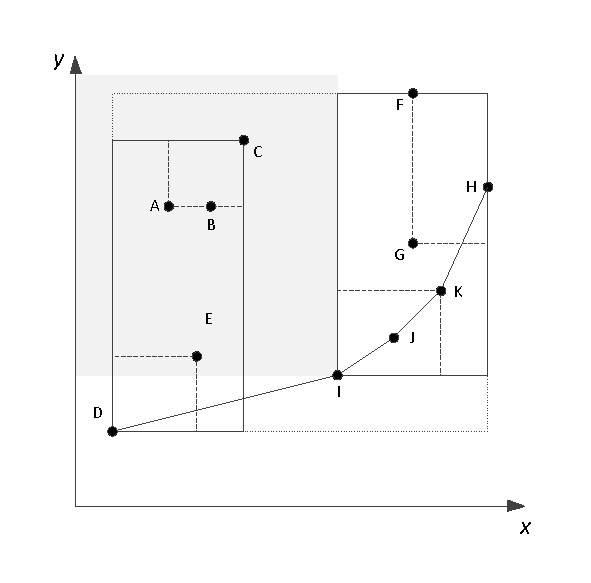
\includegraphics[width=2.5in]{Figures/skyline_maxx_miny.pdf}
\caption{\small MAX $x$, MIN $y$ and pruning region.
\label{fig:skyline_maxx_maxy}}
\end{center}
\end{figure}

\begin{figure}[h]
\begin{center}
\includegraphics[width=2.5in]{Figures/skyline_maxx_maxy.pdf}
\caption{\small MAX $x$, MAX $y$ and pruning region.
\label{fig:skyline_maxx_maxy}}
\end{center}
\end{figure}
\end{comment}


\subsection{Index-Based Skyline Pruning}

The drawback of Algorithm~\ref{alg:PBSkyline} is that the
pruning regions are formed from candidate skyline points that have
been retrieved from the broadcast channel. The pruning regions are
formed late in the program since data segments are broadcasted
after corresponding index segments.
%The reason we only use data
%records as criteria to form pruning region to accommodate
%overlapping region in index tree (such as in R-Tree).
In this section we present index-based pruning algorithm that perform
early index-based pruning and two pruning strategies that produce
the same tuning time from a client view.
The expectation is that with early pruning,
more of the index tree would be pruning and improve efficiency over
point-based pruning strategy.
%One of index structure that supports non-overlapping index regions is
%R+-Tree which can be found in ~\cite{DBLP:conf/vldb/SellisRF87}.

The two index-pruning strategies are one-region and n-regions. 
The one-region pruning strategy, forms only one pruning region per
MBR of the index tree as illustrated by Figure~\ref{fig:ibp_a}.
This strategy is based on the claim that we can prune everything from
the pivot point of the MBR of the index. The following present a short
proof of the correctness of this claim for a 2-dimensional case:

\begin{proof}
Given a 2-dimensional MBR, $r$, and skyline query of $(min, min)$.
There must exist at least one point, $p$,
in $r$ such that $p_2 = r.min_2$, $p_1$ in range
$[r.min_1, r.max_1]$. Similarly, there must exist another
point, $q$ such that $q_1 = r.min_1$, $q_2$ in range
$[r.min_2, r.max_2]$.

$p$ dominates anything to the right of $p_1$ and above
$r.min_2$ and $q$ dominates all records above $q_2$ and to
the right of $r.min_2$. We extend the $p_2$ value of the prune
region of $p$ and the $q_1$ value of the pruning region of $q$
and these two are the same as the values for the pruning region of
point $(r.min_1, r.min_2)$. Since MBRs do not overlap, pruning
regions for point $(r.min_1, b.min_2)$ is the pruning region
of the MBR $r$.
\end{proof}
Although this approach is simple, the client must keep track of the
current MBR which is inside the pruning region, but should not be
pruned. For example, MBR $A$ is inside pruning region, but it is the
MBR of the index currently being investigated. The region of $A$
should not be pruned.


n-region pruning strategy is illustrated in Figure~\ref{fig:ibp_b}.
This pruning strategy is more natural way of query evaluation. The
remaining of this section discuss the point-based skyline evaluation
algorithm using n-region strategy.

Index-Based skyline algorithm start the same way as the point-based
skyline algorithm in that initially, the pruning region is null and
the client must stay tuned to the broadcast channel until it finds
the first index bucket. When the client receives an index bucket that
is not covered by the pruning region (in this case it is the first
index bucket), it performs the following:
\begin{enumerate}
\item For each entry, create a set of $n$ pruning regions, $R'$,
    where $n$ is the dimensionality of the dataset. This is explained
    below.
\item Remove points in candidate skyline, $S$, that are covered by
    $R'$.
\item Add the new pruning regions, $R'$, to the total pruning region.
    For each $R'$, $R = R \cup R'$.
\end{enumerate}
The rationale for step 1 above to create $n$ pruning regions for each
entry is that we want prune the data dominated by the entry, but we
do not want to prune the data that is bounded by the MBR of the entry
before we download data. Figure~\ref{fig:ibp}
demonstrates this idea. Assuming the current index bucket we get from the
broadcast channel is MBR A and it is not covered by the pruning region
$R$, since MBR A is not covered, we want to follow this index to its
children $A_1$ and $A_2$ and ultimately download the data points in $A$. If we
form the pruning region of A using the strategy of Figure~\ref{fig:ibp_a},
then $A_1$ and $A_2$ will be pruned before we have the chance to download the
data. Following, the strategy of Figure~\ref{fig:ibp_b}, we have a chance
to download the data.

\begin{figure}
  \centering
  \subfigure[Pruning with one Pruning Region]{
    \label{fig:ibp_a}
    %\begin{minipage}[h!]{0.5\textwidth}
      
\includegraphics[width=1.5in]{Figures/index_based_pruning_a.eps}
    %\end{minipage}
    }
  \subfigure[Prune with $n$ Pruning Regions]{
    \label{fig:ibp_b}
    %\begin{minipage}[h!]{0.5\textwidth}
      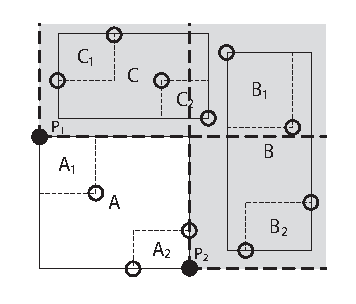
\includegraphics[width=1.5in]{Figures/index_based_pruning_b.eps}
    %\end{minipage}
    }
  \caption{Index-Based Pruning Strategies (min, min)}
  \label{fig:ibp}
\end{figure}

To create $n$ pruning regions, we need a pivot point for each pruning
region. Let $r$ be an orthotope (a MBR) and $i, j = \{1, 2, ... n\}$, such
that $p_i$ is the $i$th pivot point of $r$, and $p_{i,j}$ is the $j$th
attribute (or coordinate) of $i$th pivot point. $p_i$ is computed in the
way that $p_{i,i}$ is the opposite of $\sigma_i$ and $p_{i,j}$ is the same
as $\sigma_i$ for all $j \neq i$.

For example, for a skyline query of all MIN attributes,
$\sigma = (MIN, MIN, MIN)$ and therefore $\sigma_i = MIN$. In this case,
$p_{i,i} = r.max_i$ and $p_{i,j} = r.min_j$ for $j \neq i$.

\begin{algorithm}
\algsetup{linenosize=\small,linenodelimiter=. }
\caption{Index-Based Skyline($\sigma$)} \label{alg:IBSkyline}
\begin{algorithmic}[1]

\STATE $S \gets$ \o
\STATE $R \gets$ \o
\STATE $index \gets$ search first index segment
\STATE $queue.enqueue(index.pairs(mbr, time))$
\WHILE{$queue$ is not empty}
    \STATE $bucket \gets GetBucket(queue.dequeue)$
    \IF{$bucket$ is Index Packet}
        \FORALL{$entry \gets pair(mbr, time)$ in $bucket$}
            \IF{$R$ is not in $entry$}
                \STATE $queue.enqueue(pair)$
                \STATE $R' \gets ComputePruneRegion(e.mbr, \sigma)$
                \STATE $Prune(S, R')$
                \STATE $Prune(queue, R')$
                \STATE $R \gets R \cup R'$
            \ENDIF
        \ENDFOR
    \ELSE
        \STATE $S \gets S \cup ComputeSkyline(bucket)$
    \ENDIF
\ENDWHILE \RETURN $S$
\end{algorithmic}
\end{algorithm}

%\begin{algorithm}
%\algsetup{linenosize=\small,linenodelimiter=. }
%\caption{ComputePruneRegion($B$, $\sigma$)}
%\label{alg:ComputePruneRegion2}
%\begin{algorithmic}[1]
%\STATE $R \gets$ \o \FOR{$i = 0$ to $n$}
%    \IF{$\sigma[i] = MIN$}
%        \STATE Add dimension $i$ to $R$ from 0 to $\infty$
%    \ELSE
%        \STATE Add dimension $i$ to $R$ from 0 to $B.i_{max}$
%    \ENDIF
%\ENDFOR \RETURN $R$
%\end{algorithmic}
%\end{algorithm}

%\subsubsection{Data Preparation}
%The data and index preparation is the same as in Solution1. The only difference is that instead
%of indexing the data with R-Tree, this solution index the data with R+-Tree. The attractiveness of
%this index structure is non-overlapping MBR and we can quickly find the pruning region in our
%algorithm. Give an example of why overlapping would cause a problem.

%A drawback of this index technique is creating an R-Tree without overlapping MBRs incur
%computational overhead (cite).

\begin{comment}
\begin{figure}[h]
\begin{center}
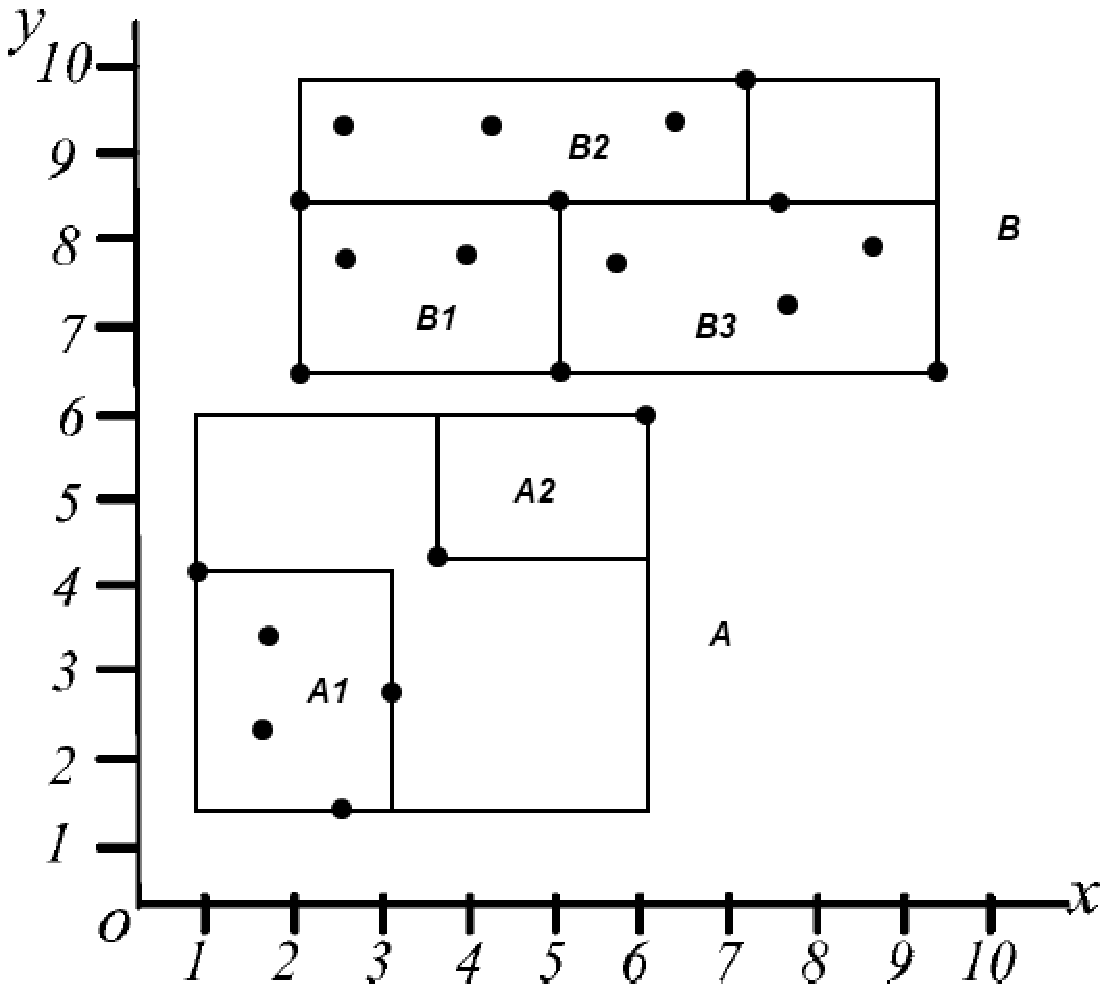
\includegraphics[width=2in]{Figures/R+Tree-eps-converted-to.pdf}
\caption{\small R+-Tree Index.\label{r+tree}}
\end{center}
\end{figure}
\end{comment}

%\subsubsection{Skyline Computation}
%
%We start with pruning region that covers space. As soon as our algorithm receives the first index
%segment we get a sense of the data distribution in space we can start forming pruning regions.
%Consider example [provide example and attach figure].  The entire index tree consists of MBRs
%A and B. Let $Min(MBR)$ be the corner of MBR that has minimum of all dimension and $Max(MBR)$
%be the corner that has maximum of all dimension. Since $Min(B)$ < $Min(A)$, we can immediately
%form the pruning region, and prune MBR A.

%Note, we don't need to consider sub-MBRs inside A and B. Since the MBRs do not overlap, the
%entire region cover by A is dominated by B. Comparing with Solution 1, we don't have to traverse
%the tree to the leaf nodes to start forming pruning regions; instead, we can obtain pruning regions
%as early as the root node of the index. This has improvement in tuning time.

%Consider all possibilities.

%\subsubsection{Correctness Verification}

%We consider the correctness of this algorithm for the MIN $x$, MIN
%$y$ case. This verification can be easily applied to other cases
%with combinations of attribute specifiers. Our goal is to prove
%the correctness of our index-based pruning algorithm. We want to
%show that we can form pruning regions from the MBR of an index
%node instead of wait until we receive data records as in
%Algorithm~\ref{alg:PBSkyline}. We also want to show that this
%algorithm does not prune false negatives (more than it should
%prune).
%
%We can form pruning region from the MBR of the index because the
%MBR of R+-Tree does not overlap. As we mentioned earlier in this
%paper, this technique does not work for index structures that
%allow overlapping index regions such as R-Tree and R*-Tree
%\cite{Beckmann:1990:RER:93597.98741}.
%
%Given a MBR, $b$, of data index that encloses data records, the
%$b$ is bounded by two points $(x_{min}, y_{min})$, $(x_{max},
%y_{max})$ and these points denote the lower-left and upper-right
%corners of the MBR respectively. There must exist a point, $p_1$,
%in $b$ such that $p_1.y = b.y_{min}$, $p_1.x$ in range
%$[b.x_{min}, b.x_{max}]$. Similarly, there must exist another
%point, $p_2$ such that $p_2.x = b.x_{min}$, $p_2.y$ in range
%$[b.y_{min}, b.y_{max}]$.
%
%$p_1$ dominates anything to the right of $p_1.x$ and above
%$b.y_{min}$ and $p_2$ dominates all records above $p_2.y$ and to
%the right of $b.x_{min}$. We extend the $y$ value of the prune
%region of $p_1$ and the $x$ value of the pruning region of $p_2$
%and these two are the same as the values for the pruning region of
%point $(b.x_{min}, b.y_{min})$. Since MBRs do not overlap, pruning
%regions for point $(b.x_{min}, b.y_{min})$ is the pruning region
%of the MBR $b$.

%\subsection{Skyline of Higher-Dimension}
%For skyline queries that involves more than two query attributes,
%we need to consider computation of skyline of higher dimension.
%Due to the generic nature of our algorithm, we can extend our
%algorithm to higher dimensions.
%
%Similar to skyline in two-dimension, we first need to index our
%data in an index structure. R-Tree and other spatial index
%structure, such as KD-Tree, can support data of arbitrary
%dimension. KD-Tree and Quad-Tree are better choice here due to
%lower computation complexity of building the index for
%higher-dimensional data. %We build our index as illustrated in Figure \ref{fig:rtree3d}.

%\begin{figure}[h]
%\begin{center}
%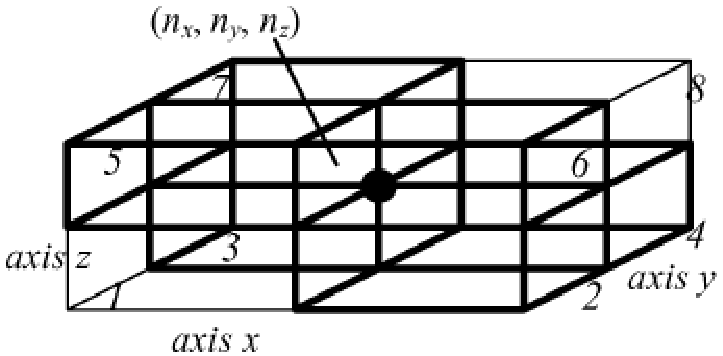
\includegraphics[width=3in]{Figures/rtree3d-eps-converted-to.pdf}
%\caption{\small Data Records inserted into R-Tree.\label{fig:rtree3d}}
%\end{center}
%\end{figure}

%Using the index, we can compute higher-dimensional pruning region
%(space) to facilitate skyline computation.

\subsection{Analysis}

This section we consider tuning time and access latency of the two
pruning region skyline algorithm we presented in this section. We
assume that the client makes skyline query at very beginning of a
cycle. Since the amount of time of time listening to the channel
is the amount of time for a client to get all desire data, the
tuning time is equal to access latency; therefore we use the same
analysis for both quantities.

We first consider the tuning time for the algorithm that uses the
point-based pruning strategy. The best case is that the client
gets all desired data from the first data segment and the rest of
the cycle is pruned. In this case, $\beta = h \times \eta +
\varsigma$. The expected case is when the client has to listen to
half of the program and $E(\beta) = \frac{1}{2}(\iota + \theta)$

We now consider the same quantity for the index-based pruning
skyline algorithm. The assumption is the same as before, but a
client does not have to traverse the index to the leaf level
before start pruning. On average, a client would have to traverse
half of the index tree but still have to download half of the
data; therefore $E(\beta) = \frac{1}{4}\iota + \frac{1}{2}\theta$
%\subsubsection{No Index}
%
%When no index is added to the broadcast cycle, the program
%length is equal to the number of data packets. The tuning time, $t_t$
%and access latency, $t_l$, is also equal to program length since a client
%have to listen to the entire broadcast cycle to compute the skyline.
%
%\begin{equation}
%    l_p = t_t = t_l = d
%\end{equation}
%
%The initial index probing time and the index percentage do not apply
%and we set both to 0.
%
%\begin{equation}
%    t_p = p_i = 0
%\end{equation}
%
%\subsubsection{One-time index}
%
%In one-time index, the index packets only appear one time at the
%beginning of the program without replication. Consider every node
%is pack in one index packet. For a full R-Tree
%index, the following defines the relationship:
%
%\begin{eqnarray}
%% \nonumber to remove numbering (before each equation)
%  h &=& \log_{b} n_t - 1 \\
%  n_i &=& \displaystyle\sum\limits_{i=0}^h b^i \\
%  l_p &=& d + n_i
%\end{eqnarray}
%
%The expected tuning time and access latency is the half of the
%broadcast program:
%
%\begin{eqnarray}
%% \nonumber to remove numbering (before each equation)
%  t_t &=& \frac{1}{2} (d + n_i) \nonumber \\
%      &=& \frac{1}{2} (d + \displaystyle\sum\limits_{i=0}^h b^i) \\
%  t_l &=& t_t
%\end{eqnarray}
%
%\subsubsection{DFDI}
%
%Assume r percent of the index is replicated and the rest is not
%replicated, the program length is as follows:
%
%\begin{equation}
%    l_p = d + (1 + r) \displaystyle\sum\limits_{i=0}^h b^i
%\end{equation}
%
%The expected tuning time and access latency is the same as for the
%one-time index that is the half of the length of the broadcast
%program. Note that, even though, the function of these two metrics
%are the same, the program length is different for both cases.
%For DFDI, since we replicated $r$ percent of the index, the program
%length is longer, therefore, the latency and tuning time are also
%longer.
